 %%%%%%%%%%%%%%%%%%%%%%% file template.tex %%%%%%%%%%%%%%%%%%%%%%%%%
%
% This is a general template file for the LaTeX package SVJour3
% for Springer journals.          Springer Heidelberg 2010/09/16
%
% Copy it to a new file with a new name and use it as the basis
% for your article. Delete % signs as needed.
%
% This template includes a few options for different layouts and
% content for various journals. Please consult a previous issue of
% your journal as needed.
%
%%%%%%%%%%%%%%%%%%%%%%%%%%%%%%%%%%%%%%%%%%%%%%%%%%%%%%%%%%%%%%%%%%%
%
% First comes an example EPS file -- just ignore it and
% proceed on the \documentclass line
% your LaTeX will extract the file if required
%!PS-Adobe-3.0 EPSF-3.0
%%BoundingBox: 19 19 221 221
%%CreationDate: Mon Sep 29 1997
%%Creator: programmed by hand (JK)
%%EndComments
%
\RequirePackage{fix-cm}

\documentclass[smallextended]{svjour3}       % onecolumn (second format)

\smartqed  
\usepackage{graphicx}       
\usepackage{longtable} 
\usepackage{amssymb,amsmath}
\usepackage{subfigure}
\usepackage{units}

\newcommand{\DuMuX}{DuMu$^\textrm{x}$}
\newcommand{\examplecommand}[1]{\textbackslash\texttt{#1}}

\begin{document}

\title{Travelling wave solutions for two-phase flow equations including hysteretic effects}

\author{T. K\"oppl \and R. Helmig \and C.J. van Duijn \and K. Mitra}
\authorrunning{K\"oppl et. al.} 

\institute{T. K\"oppl, R. Helmig \at
           University of Stuttgart, Department of Hydromechanics and Modelling of Hydrosystems, Pfaffenwaldring 61, D-70569 Stuttgart, Germany\\
           \email{\{tobias.koeppl,rainer.helmig\}@iws.uni-stuttgart.de}
           \and
           C.J. van Duijn \at
           University of Utrecht, Department of Earth Sciences, Princetonlaan 8a, 3584 CB Utrecht, Netherlands\\
           Eindhoven University of Technology, Department of Mechanical Engineering, PO Box, 5135600 MB Eindhoven, Netherlands\\
           \email{\{c.j.v.duijn\}@tue.nl}
           \and
           K. Mitra, \at
           Eindhoven University of Technology, Department of Mathematics and Computer Science, Groene loper 5, 5612 AZ Eindhoven, Netherlands\\
           Hasselt University, Faculty of Science, Martelarenlaan 42, BE3500 Hasselt, Belgium \\
           \email{\{k.mitra\}@tue.nl}
}

\date{Received: date / Accepted: date}

\maketitle

\begin{abstract}
In this work ...
\keywords{two-phase flow, hysteresis, travelling waves, Riemann problem, dynamical systems}
\end{abstract}


\section{Introduction}

\section{Mathematical model}

This section is dedicated to the formulation of a physical-mathematical model that can be used to describe an
infiltration process of a fluid into a homogeneous porous medium. An example for such an infiltration process is the
injection of water into a dry sand column (see Figure \ref{fig:column}). In the remainder of this work, we denote the absolute
permeability $K\;\left[ \unit{m}^2 \right]$ of the porous medium and its porosity by $\phi\;\left[ - \right]$.

\begin{figure}
\begin{center}
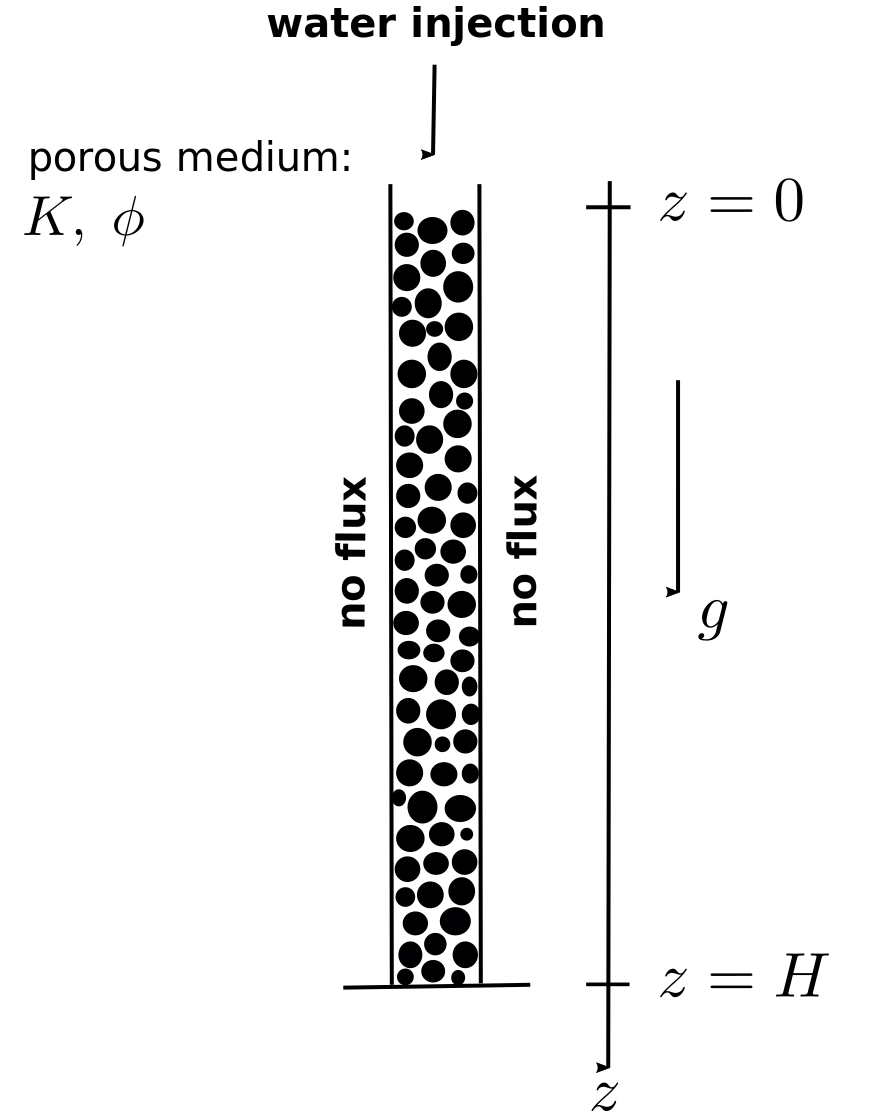
\includegraphics[width=0.5\textwidth]{column.pdf}
\end{center}
\caption{\label{fig:column} Setup of an infiltration experiment. At the inlet of a column having the height $H$ water is injected by a constant rate. The main axis
of the column is orientated such that it is aligned with the gravity vector.}
\end{figure}

\subsection{Governing equations}

For convenience, we consider in this work a one-dimenisonal two-phase flow problem defined on an interval $\left(0,H\right)$. This simplification is justified by the fact 
that the walls of a sand column in which a fluid is injected have no outflows and that the water saturation is in general almost constant across the
section area of the sand column. The interval $\left(0,H\right)$ can be considered as a parameter domain for the main axis, which is pointing into the same direction as the
gravity vector. In our one-dimenisonal flow problem $t$ and $z$, are denoting the time and space variable, respectively. Provided that there are no external source or sink terms,
the mass balance equations for the wetting phase $w$ and the non-wetting phase $n$ are given by \cite{helmig1997multiphase}:
\begin{equation}
\label{eq:massbalance}
\phi \frac{\partial\left(\rho_\alpha S_\alpha \right)}{\partial t} + \frac{ \partial \left(\rho_\alpha v_\alpha \right)}{\partial z} = 0,\; \alpha \in \left\{w,n \right\},\; z \in \left(0,H \right),\;t>0,
\end{equation}
where $S_\alpha$ and $\rho_\alpha$ represent the saturations and densities of the wetting and non-wetting phase. $v_\alpha$ denote the phase-velocities, which can be determined by 
Darcy's law:
\begin{equation}
\label{eq:Darcy}
v_\alpha = -\frac{k_{r\alpha} \left(S_w \right)}{\mu_\alpha}K \left( \frac{\partial p_\alpha}{\partial z} 
- \rho_\alpha g \right),\; \alpha \in \left\{w,n\right\}.
\end{equation}
$\mu_\alpha\;\left[Pa\cdot s\right]$ are the viscosities and $k_{r\alpha}$ are the relative permeability functions of each phase. $p_\alpha\; \left[\unit{Pa} \right]$ and 
$g\;\left[\unitfrac{m}{s^2} \right]$ stand for the phase pressures and the gravity constant. Having this notation at hand, the mobility of the phase $\alpha$ can be defined
by:
\begin{equation}
\label{eq:mobility}
\lambda_\alpha = \frac{k_{r\alpha}}{\mu_\alpha},\; \alpha \in \left\{w,n\right\}.
\end{equation}
Assuming further that the fluids are incompressible, we have constant densities:
\begin{align}
\label{eq:inkompr}
\rho_\alpha(z,t) \equiv \rho_\alpha,\; \alpha \in \left\{w,n\right\}.
\end{align}
In order to close the system, we require two constitutive relations. The first one is the saturation balance:
\begin{equation}
\label{eq:satBal}
S_w + S_n = 1
\end{equation}
and the second one is the capillary pressure relationship:
\begin{equation}
\label{eq:pc}
p_c(z,t) = p_n(z,t) - p_w(z,t),
\end{equation}
where $p_c\;\left[\unit{Pa} \right]$ is the capillary pressure. To further simplify our model, we consider the total velocity:
\begin{equation}
\label{eq:vtot}
v(z,t) = v_w(z,t) + v_n(z,t)
\end{equation}
as constant in space:
$$
\frac{\partial v}{\partial z}= 0\text{ or } v\left( z,t \right) = v \left( t \right).
$$
This assumption stems from the observation that in infiltration experiments there is often a pump injecting a fluid with a constant
flow rate and velocity into the porous medium. 
In order to account for the different flow behavior during an imbibition or drainage
process, we consider the non-equilibrium model combining dynamic effects in the $p_c-S_w$, $k_{rw}-S_w$ and $k_{rn}-S_w$ relationships with a 
simple, play-type hysteresis model \cite{morrow1965capillary,plohr2001modeling,schneider2018stable}. A mathematical derivation of the play-type hysteresis model for the
capillary pressure the pore scale analysis can be found in \cite{beliaev2001theoretical}.
As a first step towards a play-type hysteresis model, we introduce for the capillary pressure and the relative permeabilities a specific function, 
for both the drainage $\left(d \right)$ and imbibition process $\left(i \right)$:
\begin{equation}
\label{eq:dynamic}
\zeta \left( S_w \right)=
\begin{cases}
 \zeta^{(i)}\left( S_w \right),\text{ if } \frac{\partial S_w}{\partial t} \geq 0, \\
 \\
 \zeta^{(d)}\left( S_w \right),\text{ if } \frac{\partial S_w}{\partial t} < 0,
\end{cases} \text{ for }
\zeta \in \left\{ p_c,\;k_{rw},\;k_{rn}\right\}.
\end{equation}
Combining \eqref{eq:dynamic} with the vertical scanning curves, one obtains the following closure relationship:
\begin{equation}
\label{eq:closure}
\zeta\left( S_w,\frac{\partial S_w}{\partial t} \right) 
\in \zeta^+\left( S_w \right) - \zeta^-\left( S_w \right) \cdot \text{sign} \left( \frac{\partial S_w}{\partial t} \right),\;\zeta \in \left\{ p_c,\;k_{rw},\;k_{rn}\right\}.
\end{equation}
By $\text{sign}$, we denote the multi-valued signum graph:
$$
\text{sign} \left( \xi \right) = 
\begin{cases}
 1, &\text{ for } \xi > 0,\\
 \left[-1,1 \right], &\text{ for } \xi = 0,\\
 -1, & \text{ for } \xi < 0.
\end{cases}
$$
The functions $\zeta^+$ and $\zeta^-$ are defined as follows:
$$
\zeta^+\left( S_w \right) = \frac 12 \left( \zeta^{(d)}\left( S_w \right) + \zeta^{(i)}\left( S_w \right) \right) \text{ and } 
\zeta^-\left( S_w \right) = \frac 12 \left( \zeta^{(d)}\left( S_w \right) - \zeta^{(i)}\left( S_w \right) \right).
$$
Concerning the main imbibition and drainage curves that occur in the hysteresis model, we make the following assumptions:
\ \\
\begin{itemize}
 \item[(A1)] $k_{rw}^{\left(k \right)} \in C^1\left( \left[0,1 \right] \right),\;k_{rw}^\prime\left( S_w \right)>0$ for $0<S_w \leq 1,\;k_{rw}^{\left(k \right)}\left( 0 \right) = 0$
 and $k_{rw}^{\left( k \right)},\;k \in \left\{ i,d \right\}$ are strictly convex.\\
 \\
 \item[(A2)] $k_{rn}^{\left(k \right)} \in C^1\left( \left[0,1 \right] \right),\;k_{rn}^\prime\left( S_w \right)<0$ for $0 \leq S_w < 1,\;k_{rn}^{\left(k \right)}\left( 1 \right) = 0$
 and $k_{rn}^{\left( k \right)},\;k \in \left\{ i,d \right\}$ are strictly convex.\\
 \\
 \item[(A3)] The capillary pressure functions $p_c^{\left(k \right)},\;k \in \left\{ i,d \right\}$ fulfill: 
 $$
 p_c^{\left(k \right)}: \left(0,1 \right] \rightarrow \left[0,\infty \right),\;p_c^{\left(k \right)} \in C^1\left( \left( 0,1 \right] \right),
 $$
 $p_c^{\left(k \right)} \left( 1 \right) = 0,\; \left( p_c^{\left(k \right)} \right)^\prime\left(S_w \right) < 0$ and $p_c^{\left( i \right)}\left(S_w \right) < p_c^{\left( d \right)}\left(S_w \right)$ for
 $S_w \in \left(0,1 \right)$.
\end{itemize}
\ \\
Please note that the superscript $\prime$ represents the differentiation with respect to the argument of the respective function.

\subsection{Dimensionless formulation}
From Darcy's law \eqref{eq:Darcy}, \eqref{eq:pc} and \eqref{eq:vtot} one finds:
$$
v_w = \frac{\lambda_w}{\lambda_n + \lambda_w} v + K \frac{\lambda_n \lambda_w}{\lambda_n + \lambda_w} \left( \frac{ \partial p_c }{ \partial z} + \left(\rho_w-\rho_n \right)g \right).
$$
Substituting this relationship into \eqref{eq:massbalance} for $\alpha = w$ gives the transport equation for the wetting phase:
$$
\frac{\partial S}{\partial t} + \frac{v}{\phi} \frac{\partial}{\partial z} \left[ \frac{\lambda_w}{\lambda_n + \lambda_w} +
\frac{K \left(\rho_w-\rho_n \right) g}{v} \frac{\lambda_n \lambda_w}{\lambda_n + \lambda_w} + \frac{K}{v}\frac{\lambda_n \lambda_w}{\lambda_n + \lambda_w}
\frac{\partial p}{\partial z} \right] = 0,
$$
where from now on, we use the following notation: $S = S_w$ and $p = p_c$. Introducing the fractional flow function:
$$
f\left(S \right) = \frac{\lambda_w}{\lambda_n + \lambda_w} = \frac{k_{rw}}{k_{rw}+ \frac{\mu_w}{\mu_n}k_{rn}}
$$
and the function 
$$
h\left(S \right) = \frac{k_{rn} k_{rw}}{k_{rw} + \frac{\mu_w}{\mu_n} k_{rn}} = k_{rn}\left(S \right) f\left(S \right)
$$
one obtains:
$$
\frac{\lambda_n \lambda_w}{\lambda_n + \lambda_w} = \frac{1}{\mu_n} h\left( S \right).
$$
Let $z_r\;\left[\unit{m} \right]$ be a characteristic length, $p_r\;\left[\unit{Pa} \right]$ a characteristic pressure and
$t_r = \frac{\phi z_r}{v}$ a characteristic time. Setting
$$
z^\ast := \frac{z}{z_r},\quad t^\ast := \frac{t}{t_r},\quad p^\ast := \frac{p}{p_r}
$$
and defining the dimensionless numbers
$$
N_g := \frac{K\left(\rho_w - \rho_n \right) g}{v \mu_n}\;\text{(gravity number) and }
N_c : = \frac{K p_r}{v \mu_n z_r}\;\text{(capillary number)}
$$
yields the dimensionless transport equation:
$$
\frac{\partial S}{\partial t^\ast} +  \frac{\partial}{\partial z^\ast}\left( f\left(S \right) + N_g h\left(S \right) + N_c h\left(S \right) \frac{\partial p^\ast}{\partial z^\ast} \right) = 0.
$$
Please note that for convenience, we will omit the asterisks in the remainder of this work:
\begin{equation}
\label{eq:dimlessTE}
\frac{\partial S}{\partial t} +  \frac{\partial}{\partial z}\left( f\left(S \right) + N_g h\left(S \right) + N_c h\left(S \right) \frac{\partial p}{\partial z} \right) = 0.
\end{equation}
In conformity with \eqref{eq:closure} the hysteresis functions for the dimensionless formulation \eqref{eq:dimlessTE} read as follows:
\begin{equation}
\label{eq:hysteresis_pfh}
\zeta \left( S, \frac{\partial S}{\partial t} \right) \in \zeta^+\left( S \right) - \zeta ^-\left( S \right) \cdot \text{sign} \left( \frac{\partial S}{\partial t} \right),\; 
\zeta \in \left\{ p,f,h \right\}.
\end{equation}
Instead of the multi-valued function $\text{sign}$, we use for our analysis a regularization of this function. Let $\epsilon>0$ be a small regularization parameter
and $\text{sign}_\epsilon$ the regularization of $\text{sign}$, which satifies a further assumption:
\;
\begin{itemize}
 \item[(A4)] For each $\epsilon >0$, $\text{sign}_\epsilon$ is strictly monotonous and piecewise smooth. Furthermore it holds:
 $$
 \text{sign}_\epsilon \left( -\xi \right) = \text{sign}_\epsilon \left( -\xi \right) \text{ and } 0 < \text{sign}_\epsilon^\prime \left(S_w \right) \leq 
 \text{sign}_\epsilon^\prime\left(0 \right) =  \frac{1}{\epsilon}, \; \forall \xi \in \mathbb{R}
 $$
 and
 $$
 \lim_{\xi \rightarrow \pm \infty} \text{sign}_\epsilon \left( \xi \right) = \pm 1,\qquad \lim_{\epsilon \rightarrow 0}\text{sign}_\epsilon \left( 0 \right) 
 = 
 \begin{cases}
  -1, &\text{ if } \xi < 0,\\
  +1, &\text{ if } \xi > 0.
 \end{cases}
 $$
 $\text{sign}_\epsilon$ depends smoothly and monotonically on $\epsilon$, i.e. for $0<\epsilon_2<\epsilon_1$ it holds: 
 $\left| \text{sign}_{\epsilon_1} \left( \xi \right) \right| < \left| \text{sign}_{\epsilon_2} \left( \xi \right) \right|, \; \forall \xi \neq 0.$
The inverse function of $\text{sign}_\epsilon$ is denoted by $\Psi_\epsilon$ in the remainder of this manuscript.
\end{itemize}
\;
Using \eqref{eq:hysteresis_pfh} and the regularization in (A4) we have the following modified hysteresis model:
\begin{equation}
\label{eq:hysteresis_pfh_reg}
\zeta \left( S, \frac{\partial S}{\partial t} \right) \in \zeta^+\left( S \right) - \zeta ^-\left( S \right) \cdot \text{sign}_\epsilon \left( \frac{\partial S}{\partial t} \right),\; 
\zeta \in \left\{ p,f,h \right\}.
\end{equation}
From \eqref{eq:hysteresis_pfh_reg}, it follows for the case $\zeta = p$:
\begin{equation*}
-1 \leq \frac{p^+-p}{p^-} = \text{sign}_\epsilon \left( \frac{\partial S}{\partial t} \right) \leq 1.
\end{equation*}
By this, we obtain:
\begin{equation*}
\chi \left( S, p \right) \in \chi^+\left( S \right) - \chi^-\left( S \right) \cdot \left( \frac{p_c^+\left( S \right) -p}{p_c^-\left( S \right)} \right),\; \chi \in \left\{ f,h \right\}.
\end{equation*}
Taking this relationship into account, one can rewrite the transport equation \eqref{eq:dimlessTE} combined with the inverse function $\Psi_\epsilon$ from (A4):
\begin{align}
\label{eq:TE}
\frac{\partial S}{\partial t} +  \frac{\partial}{\partial z}\left( f\left(S,p \right) + N_g h\left(S,p \right) + N_c h\left(S,p \right) \frac{\partial p}{\partial z} \right) &= 0, \\
\nonumber
\\
\label{eq:hyst_psi}
\frac{\partial S}{\partial t} -  \Psi_\epsilon \left( \frac{p_c^+\left( S \right) -p}{p_c^-\left( S \right)} \right) &= 0.
\end{align}

\section{Analysis of the travelling wave formulation}

Having derived the non-dimensional hysteretic two-phase flow system \eqref{eq:TE} and \eqref{eq:hyst_psi} in the previous section, we investigate in this section under 
which conditions travelling wave solutions can be observed for this PDE system. Thereby, we assume that \eqref{eq:TE} and \eqref{eq:hyst_psi} are defined on $\mathbb{R}$
with respect to the spatial variable $z$. The initial condition for the saturation $S$ is given by: 
$$
S \left(z,0 \right) = 
\begin{cases}
S_l,\;\text{ for } z < 0, \\
S_r,\;\text{ for } z \geq 0.
\end{cases}
$$
Corresponding to the saturation values $S_l$ and $S_r$, there are pressure values $p_l$ and $p_r$, which are chosen such that the following holds $\forall t>0$:
\begin{align}
\label{eq:pairs}
\left( S\left(z,t \right), p\left(z,t\right) \right) &\rightarrow \left(S_l,p_l \right)\;  \text{ for } \; z \rightarrow -\infty, \\
\nonumber
\left( S\left(z,t \right), p\left(z,t\right) \right) &\rightarrow \left(S_r,p_r \right)\; \text{ for } \; z \rightarrow  \infty.
\end{align}
Using this notation, the issue under consideration reads as follows: Which pairs $\left\{S_l,p_l \right\}$ and $\left\{S_r,p_r \right\}$ can  be connected by a viscous profile, i.e., we want to investigate,
whether there is a travelling wave solution of \eqref{eq:TE} and \eqref{eq:hyst_psi} that satisfies \eqref{eq:pairs}. A first step to investigate this issue, is to combine the travelling wave ansatz
\begin{equation}
\label{eq:ansatz}
S\left(z,t \right) = S\left( \xi \right),\; p\left(z,t \right) = p\left( \xi \right)\;\text{ with }\;\xi = ct-z
\end{equation}
with the hysteretic two-phase flow model \eqref{eq:TE} and \eqref{eq:hyst_psi}. In \eqref{eq:ansatz}, $S$ and $p$ are travelling wave profiles and $c$ the corresponding wave speed. Substituting
\eqref{eq:ansatz} into \eqref{eq:TE} and \eqref{eq:hyst_psi} yields:
\begin{subequations}
\begin{equation}
\label{eq:ODES1}
cS^\prime - \left(  f\left(S,p \right) + N_g h\left(S,p \right) + N_c h\left(S,p \right)p^\prime \right)^\prime = 0, 
\end{equation}
\begin{equation}
\label{eq:ODES2}
cS^\prime =  \Psi_\epsilon \left( \frac{p^+\left( S \right) -p}{p^-\left( S \right)} \right), 
\end{equation}
\end{subequations}
for $\xi \in \mathbb{R}$. Integrating \eqref{eq:ODES1}, one obtains:
$$
cS - \left(  f\left(S,p \right) + N_g h\left(S,p \right) + N_c h\left(S,p \right)p^\prime \right) = A.
$$
Assuming that $p^\prime\left( \xi \right) = 0$ for $\xi \gg 1$ and applying the limits $\xi \rightarrow \pm \infty$ in the previous equation, we have
by means of the boundary conditions:
\begin{align*}
c S_l - f_l -N_g h_l &= A, \\
c S_r - f_r -N_g h_r &= A,
\end{align*}
where
$$
\zeta_l = \zeta \left( S_l,p_l \right),\; \zeta_r = \zeta \left( S_r,p_r \right),\; \zeta \in \left\{ f,h \right\}.
$$
Solving the above system of equations, for $c$ and $A$, yields a Rankine-Hugoniot condtion for $c$:
$$
c = \frac{\left(f_r +N_g h_r \right) - \left(f_l +N_g h_l \right)}{S_r-S_l}
$$
and
$$
A = cS_l - \left(f_l +N_g h_l \right) = cS_r - \left(f_r +N_g h_r \right).
$$
By this, the travelling wave formulation of the hysteretic two-phase flow system \eqref{eq:TE} and \eqref{eq:hyst_psi} is given by:
\begin{subequations}
\begin{equation}
\label{eq:ODES} 
S^\prime = \frac{1}{c} \Psi_\epsilon \left( \frac{p_c^+\left( S \right) -p}{p_c^-\left( S \right)} \right),
\end{equation}
\begin{equation}
\label{eq:ODEp}
p^\prime = \frac{1}{N_c h\left(S,p \right)} \left( A- cS + f\left(S,p\right) + N_g h\left(S,p\right)  \right). 
\end{equation}
\end{subequations}
Defining the hysteretic region $H$ by:
$$
H = \left\{ \left(S,p \right) \left|\; 0<S<1,\;p_c^{(i)}\left(S \right) < p < p_c^{(d)}\left(S \right) \right. \right\}
$$
it follows directly for \eqref{eq:ODES}:
\begin{align*}
cS^\prime > 0 \text{ in } H^- =  \left\{ \left(S,p \right) \left| \;0<S<1,\;p_c^{(i)}\left(S \right) < p < p_c^+\left(S \right) \right. \right\}, \\
\ \\
cS^\prime < 0 \text{ in } H^+ =  \left\{ \left(S,p \right) \left| \;0<S<1,\;p_c^{+}\left(S \right) < p < p_c^{(d)}\left(S \right) \right. \right\},
\end{align*}
where the capillary pressure curves are given in a dimensionless form in this context. Concerning the boundary conditions $\left(S_l,p_l \right)$ and
$\left( S_r,p_r \right)$ we further assume that they are equilibrium points of the system \eqref{eq:ODES} and \eqref{eq:ODEp}. From \eqref{eq:ODES}
one can conclude that for consistency it has to hold:
$$
\Psi_\epsilon \left|_{S_l,p_l}  = 0 \right. \Leftrightarrow p_l = p_c^+\left(S_l \right) \; \text{ and } \;
\Psi_\epsilon \left|_{S_r,p_r} = 0 \right. \Leftrightarrow p_r = p_c^+\left(S_r \right).
$$
Therefore, we use the following equilibrium points:
$$
E_l = \left(S_l,  p_l = p_c^+\left(S_l \right) \right) \;\text{ and }\; E_r = \left(S_r,  p_r = p_c^+\left( S_r \right) \right).
$$
In the remainder of this section we discuss the properties of these equilibrium points in terms of the dynamical system \eqref{eq:ODES} and \eqref{eq:ODEp}. 
Thereby, in a first step the cases without the gravity term, i.e., $N_g = 0$ is discussed, while in the other case the influence of the gravity term is taken into 
account.

\subsection{Case 1: $N_g = 0$}

In this case, the dynamical system \eqref{eq:ODES} and \eqref{eq:ODEp} is reduced to:
\begin{subequations}
\begin{equation}
\label{eq:ODESng} 
S^\prime = \frac{1}{c} \Psi_\epsilon \left( \frac{p_c^+\left( S \right) -p}{p_c^-\left( S \right)} \right),
\end{equation}
\begin{equation}
\label{eq:ODEpng}
p^\prime = \frac{1}{N_c h\left(S,p \right)} \left( A- cS + f\left(S,p\right) \right) =: G\left(S,p \right)
\end{equation}
\end{subequations}
and the parameters $c$ and $A$ are given by:
$$
c = \frac{f_r-f_l}{S_r-S_l}\;\text{ and }\;A = c S_l -f_l = c S_r -f_r,
$$
where we used the following notation:
$$
\zeta_\alpha = \zeta \left(S_\alpha,p_\alpha \right) = \zeta_\alpha \left( S_\alpha,p_c^+\left( S_\alpha \right) \right) = \zeta^+\left( S_\alpha \right),\; \alpha \in \left\{r,l \right\},\;\zeta \in \left\{ f,h \right\}.
$$
For $S_r>S_l$ and taking into account that $f^+$ is monotonously increasing, it is obvious that $c>0$ and therefore it holds:
$$
S^\prime > 0 \text{ in } H^- \;\text{ and }\; S^\prime < 0 \text{ in } H^+.
$$
In order to investigate the nature of the equilibirum points $E_l$ and $E_r$, we linearize the right hand sides of \eqref{eq:ODESng}  and \eqref{eq:ODEpng}.
Computing the partial derivatives of these functions for $p=p_c^+\left( S \right)$, we obtain for $\alpha \in \left\{r,l \right\}$:
\begin{align*}
\left. \frac{\partial \Psi_\epsilon}{\partial S}\right|_{E_\alpha}  &=\frac{1}{c} \Psi^\prime_\epsilon \left(0 \right) \frac{ \left( p_c^+\left( S_\alpha \right) \right)^\prime }{ p_c^-\left( S_\alpha \right) },
\quad \left.\frac{\partial \Psi_\epsilon}{\partial p}\right|_{E_\alpha} = -\frac{1}{c} \Psi^\prime_\epsilon \left(0 \right) \frac{ 1 }{ p_c^-\left( S_\alpha \right) }, \\
\ \\
\left. \frac{\partial G}{\partial S} \right|_{E_\alpha} &= \frac{1}{N_ch^+\left( S_\alpha \right)}\left( \left. \frac{\partial f}{\partial S} \right|_{E_\alpha} -c \right),\quad 
\left. \frac{\partial G}{\partial p} \right|_{E_\alpha}= \frac{1}{N_ch^+\left( S_\alpha \right)} \frac{f^-\left( S_\alpha \right)}{p_c^-\left( S_\alpha \right)}.
\end{align*}
Since
$$
\left. \frac{\partial f}{\partial S}  \right|_{E_\alpha} = \left( f^+\left( S_\alpha \right) \right)^\prime - f^-\left( S_\alpha \right) \frac{\left( p_c^+\left( S_\alpha \right) \right)^\prime }{p_c^-\left( S_\alpha \right)},
$$
the derivate for $G$ with respect to $S$ reads as:
$$
\left. \frac{\partial G}{\partial S}  \right|_{E_\alpha} = \frac{1}{N_ch^+ \left( S_\alpha \right)}\left(  \left( f^+\left( S_\alpha \right) \right)^\prime -c  - f^- \frac{\left( p_c^+\left( S_\alpha \right) \right)^\prime }{p_c^-\left( S_\alpha \right)} \right)
$$
Observing that $\Psi_\epsilon^\prime \left(0 \right) = \epsilon$ (see assumption (A4)), we further conclude using $ \left( p_c^+ \left(S \right) \right)^\prime <0$:
\begin{align*}
\left. \frac{\partial \Psi_\epsilon}{\partial S}\right|_{E_\alpha}  &= -c_1\left( E_\alpha \right) \epsilon,\quad c_1\left( E_\alpha \right) = - \frac{1}{c}  
\frac{ \left( p_c^+ \left(S_\alpha \right) \right)^\prime }{ p_c^- \left(S_\alpha \right) } > 0, \\
\left. \frac{\partial \Psi_\epsilon}{\partial p}\right|_{E_\alpha}  &= -c_2\left( E_\alpha \right) \epsilon,\quad c_2\left( E_\alpha \right) = \frac{1}{c}  
\frac{1}{ p_c^- \left(S_\alpha \right) } > 0, \\
\left. \frac{\partial G}{\partial S} \right|_{E_\alpha} &= c_3\left( E_\alpha \right),\quad 
c_3\left( E_\alpha \right) =  \frac{1}{N_ch^+\left( S_\alpha \right)} \left(  \left( f^+\left( S_\alpha \right) \right)^\prime - c - 
 \underbrace{\left. \frac{ f^- \left( p_c^+ \right)^\prime}{p_c^-} \right|_{S_\alpha}}_{>0} \right), \\
\left. \frac{\partial G}{\partial p} \right|_{E_\alpha} &= c_4\left( E_\alpha \right),\quad c_4\left( E_\alpha \right) = \frac{1}{N_c}
\left. \frac{f^-}{h^+ p_c^-} \right|_{S_\alpha} >0.
\end{align*}
Finally, the eigenvalues of the Jacobian associated with the mapping
$$
\begin{pmatrix} S \\ p \end{pmatrix} \mapsto 
\begin{pmatrix} \frac{1}{c} \Psi_\epsilon\left(S,p \right) \\ G\left(S,p \right) \end{pmatrix}
$$
are given by:
$$
\lambda_{pm} = \frac{1}{2}\left( c_4 - \epsilon c_1 \right) \pm \frac{1}{2} \left| c_4 - \epsilon c_1 \right|
\sqrt{ 1- \frac{4 \epsilon c_2 c_3}{\left( c_4-\epsilon c_1\right)^2} }.
$$
Choosing $\epsilon>0$ sufficiently small, the term for the eigenvalues may be rewritten as follows:
$$
\lambda_{pm} = \frac{1}{2} \left( c_4 - \epsilon c_1 \right) \left( 1 \pm \sqrt{ 1- \frac{4 \epsilon c_2 c_3}{\left( c_4-\epsilon c_1\right)^2}} \right).
$$
Based on this second term, it can be observed that:
\begin{align*}
c_3>0 &\Rightarrow 0 < \lambda_- < \lambda_+,\;\Rightarrow \text{ unstable equilibrium point}, \\
c_3<0 &\Rightarrow \lambda_- < 0 < \lambda_+,\;\Rightarrow \text{ equilibrium saddle point}.
\end{align*}
Hence, if $S_r$ and $S_l$ are chosen such that:
$$
c_3\left( E_l \right) = \left( f^+\left( S_l \right) \right)^\prime - c - \left. \frac{ f^- \left( p_c^+ \right)^\prime}{p_c^-} \right|_{S_l} > 0,
$$
then a solution orbit can never reach $E_l$ for $\xi \rightarrow -\infty$. In the other case, if $S_r$ and $S_l$ are chosen such that:
$$
c_3\left( E_l \right) = \left( f^+\left( S_l \right) \right)^\prime - c - \left. \frac{ f^- \left( p_c^+ \right)^\prime}{p_c^-} \right|_{S_l} < 0,
$$
then $E_l$ is a saddle point and a connecting orbit might be possible.

\subsection{Case 2: $N_g \neq 0$}

\section{Numerical results}

\section{Final remarks}


\begin{acknowledgements}
This work was partially supported by the Cluster of Excellence in Simulation Technology (EXC 310/2).
\end{acknowledgements}

\bibliographystyle{plain}     
\bibliography{Literature}  
\nocite{*}

\end{document}
